\documentclass[twoside,a4paper]{article}
\usepackage{geometry}
\geometry{margin=1.5cm, vmargin={0pt,1cm}}
\setlength{\topmargin}{-1cm}
\setlength{\paperheight}{29.7cm}
\setlength{\textheight}{25.3cm}

% useful packages.
\usepackage{amsfonts}
\usepackage{amsmath}
\usepackage{amssymb}
\usepackage{amsthm}
\usepackage{enumerate}
\usepackage{graphicx}
\usepackage{multicol}
\usepackage{fancyhdr}
\usepackage{layout}
\usepackage{float}

% some common command
\newcommand{\dif}{\mathrm{d}}
\newcommand{\avg}[1]{\left\langle #1 \right\rangle}
\newcommand{\difFrac}[2]{\frac{\dif #1}{\dif #2}}
\newcommand{\pdfFrac}[2]{\frac{\partial #1}{\partial #2}}
\newcommand{\OFL}{\mathrm{OFL}}
\newcommand{\UFL}{\mathrm{UFL}}
\newcommand{\fl}{\mathrm{fl}}
\newcommand{\op}{\odot}
\newcommand{\Eabs}{E_{\mathrm{abs}}}
\newcommand{\Erel}{E_{\mathrm{rel}}}

\begin{document}

\pagestyle{fancy}
\fancyhead{}
\lhead{Jovi Wong(3180104829)}
\chead{Math Software \#day2}
\rhead{2020/7/7}
\section*{I. Summary}

\subsection*{1.plot}

\Large{DATA} \\
At least one paired vectors with the same length.\\
\\
\Large{STYLE}\\

\begin{tabular}{cc|cc|cc}
\hline
color & character & marker & symbol& line & symbol  \\
\hline
yellow & y & circle & o & solid & -\\
magenta & m & Plus sign & + & dashed & --\\
cyan & c & Asterisk & * & dotted & :\\
red & r & Point & . & dash-dot & -.\\
green & g & Cross & x\\ 
blue & b & Square & s\\ 
white & w & Diamond & d\\
black & k & Pentagram & p\\
 &  & Hexagram & h\\
\end{tabular}
\\
\\
\Large{ARGUMENT}\\

\begin{tabular}{|c|c|}
\hline
keyword & description \\
\hline
'Color' & line color\\
'LineStyle' & line style \\
'LineWidth' & line width \\
'Marker' & Marker Symbol \\
'MarkerEdgeColor' & Marker outline color\\
'MarkerFaceColor' & Marker fill color\\
\hline
\end{tabular}\\
\vbox{}\vbox{}\vbox{}\\
\Large{EXPANSION}\\
Function plot3 can display 3D curve receiving three vectors with the same length. Besides, we can use ezplot to plot implicit function.
\subsection*{2.bar}
\Large{DATA}\\
One Vector: horizontal cordinate is natural number and longitudinal cordinate is value. \\
Two Vector: horizontal cordinate represents values in the first vector and longitudinal cordinate is the second vector.\\
Matrix : display data in each column by group.\\
\\
\Large{STYLE}\\
'grouped':Display each group as adjacent bars that are centered around their corresponding x value.\\
'stacked':Display each group as one multicolored bar. The length of a bar is the sum of the elements in the group. If y is a vector, then the result is the same as 'grouped'.\\
'histc':Display the bars in histogram format, in which the bars in a group touch one another. The trailing edge of each group is aligned with the corresponding x value.\\
'hist':Display the bars in histogram format. Each group is centered at the corresponding x value.\\
\\
\Large{ARGUMENT}\\

\begin{tabular}{|c|c|}
\hline
keyword & description \\
\hline
'BaseValue' & baseline value\\
'LineStyle' & Line style of bar outlines \\
'LineWidth' & Width of bar outlines\\
b & Bar objects\\
\hline
\end{tabular}
\subsection*{3.mesh}
\Large{DATA}\\
 The function plots the values in matrix Z as heights above a grid in the x-y plane defined by X and Y. The edge colors vary according to the heights specified by Z. Matrixes X and Y come from vector x and y which represent the way to divide cordinates.\\
\\
\Large{INPUT}\\
x-coordinates specified as a matrix the same size as Z, or as a vector with length n, where [m,n] = size(Z). If you do not specify values for X and Y, mesh uses the vectors (1:n) and (1:m).\\
y-coordinates, specified as a matrix the same size as Z or as a vector with length m, where [m,n] = size(Z). If you do not specify values for X and Y, mesh uses the vectors (1:n) and (1:m).\\
z-coordinates specifies the height of the mesh plot at each x-y coordinate. If you do not specify the colors, then Z also specifies the mesh edge colors.\\
Color array, specified as an m-by-n matrix of colormap indices or as an m-by-n-by-3 array of RGB triplets, where Z is m-by-n.\\
To use colormap colors, specify C as a matrix. For each grid point on the mesh surface, C indicates a color in the colormap. The CDataMapping property of the surface object controls how the values in C correspond to colors in the colormap.\\
\Large{ARGUMENT}\\

\begin{tabular}{|c|c|}
\hline
keyword & description \\
\hline
'EdgeColor'  & Edge line color\\
'LineStyle' & Line style \\
'FaceColor'  & Face color\\
'FaceAlpha' & Face transparency\\
'FaceLighting' & Effect of light objects on faces\\
\hline
\end{tabular}\\
\\
\Large{EXPANSION}\\
Function the syntax of surf is quite similar to function mesh but with color on the surface of the object. In addition, we can set light from certain angle.
\section*{II. Questions in Handouts}
\subsection*{Plot two cylinders with the same radius cross each other}
\Large{CODE}\\
\\
$[x,y,z]$ = cylinder(1,50);\\
surf(x,y,z);\\
axis square;\\
hold on\\
$[x1,y1,z1]$ = cylinder(1,50);\\
z1 = z1 - 0.5;\\
y1 = y1 +0.5;\\
surf(z1,x1,y1);\\
hold off\\
\Large{PICTURE}
\begin{figure}[b]
\centering
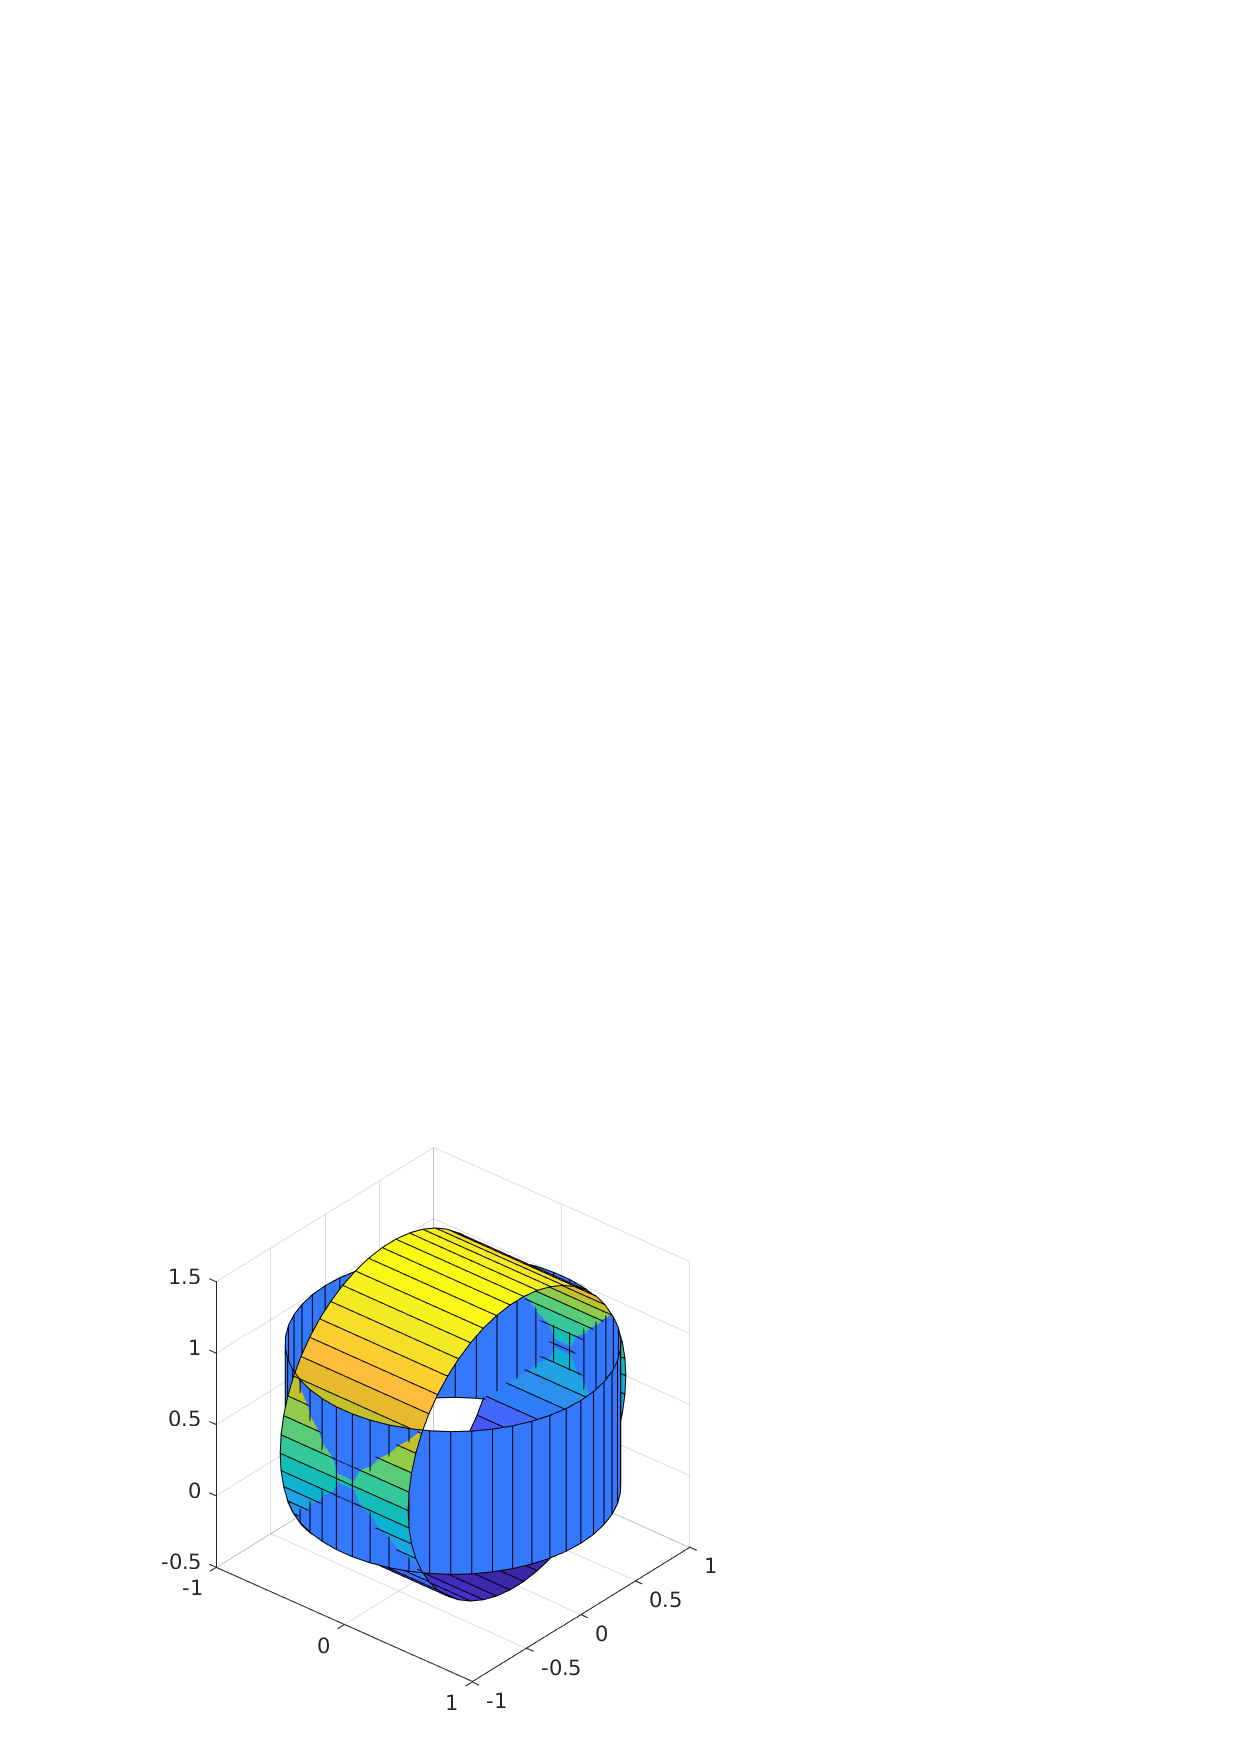
\includegraphics[width=4in]{2Cylinder.jpg}
\end{figure}

\subsection*{Julia Set}
\begin{figure}[H]
\centering
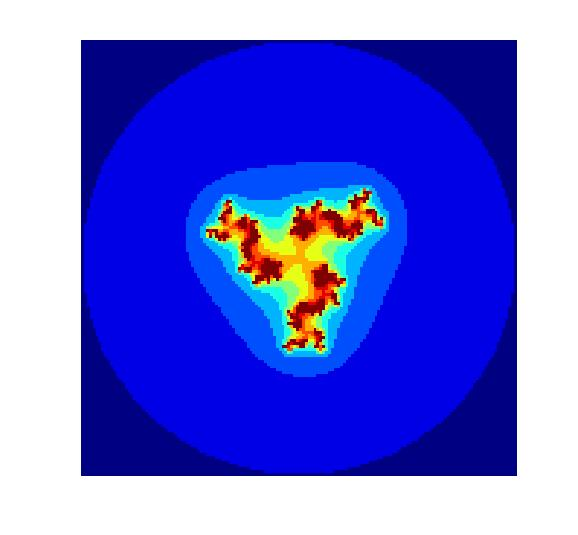
\includegraphics[width=4in]{julia3.jpg}
\caption{Iterate using a cubic equation}
\end{figure}
\begin{figure}[H]
\centering
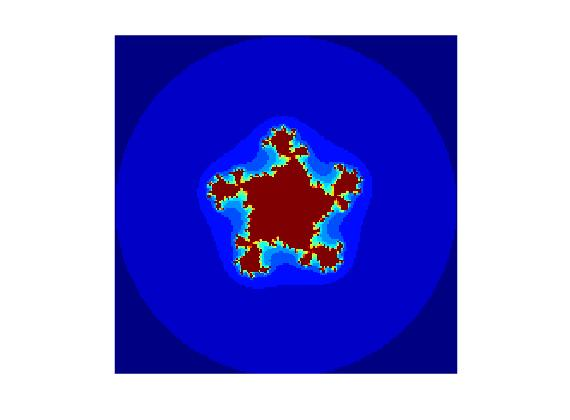
\includegraphics[width=5in]{julia5.jpg}
\caption{Iterate using a quintic equation}
\end{figure}

\end{document}

%%% Local Variables: 
%%% mode: latex
%%% TeX-master: t
%%% End: 
